% 开普勒第二和第三定律的证明
% 开普勒第二定律|开普勒第三定律|轨道周期

\pentry{开普勒三定律\upref{Keple}}

\subsection{第二定律}
\begin{figure}[ht]
\centering
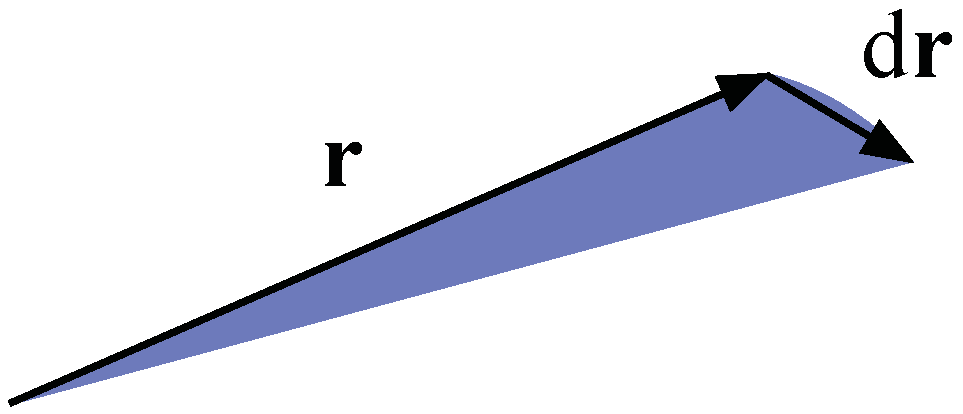
\includegraphics[width=4.5cm]{./figures/Keple21.pdf}
\caption{微小时间 $\dd{t}$ 内位矢扫过的面积} \label{Keple2_fig1}
\end{figure}

令质点的位矢为 $\vec r$,  在很小一段时间 $\dd{t}$ 内移动了 $\dd{\vec r}$,  于是位矢扫过的面积就是以 $\vec r$ 和 $\dd{\vec r}$ 为两条边的三角形的面积
\begin{equation}
\dd{S} = \abs{\vec r} \abs{\dd{\vec r}} (\sin \theta) /2
\end{equation}
其中 $\theta$ 为两条矢量的夹角.若把面积看成矢量, 方向垂直于三角形所在的平面, 则根据叉乘的定义有 $\dd{\vec S} = \vec r \cross \dd{\vec r/2}$. 两边除以 $\dd{t}$,  得扫过面积的速率为
\begin{equation}
\dv{\vec S}{t} = \frac12 \vec r \cross \dv{\vec r}{t} = \frac12 \vec r\cross \vec v = \frac{\vec L}{2m}
\end{equation}
其中 $\vec L$ 是质点的轨道角动量. 我们已知在中心力场问题\upref{CenFrc} 中, 角动量守恒. 把上式记为标量形式, 即
\begin{equation}\label{Keple2_eq3}
\dv{S}{t} = \frac{L}{2m}
\end{equation}
这说明面积 $S$ 随时间增加的速率为常数. 证毕.

\subsection{第三定律}
我们要试图找到开普勒问题中椭圆轨道的周期与其形状大小之间的关系. 一个直接的思路就是用椭圆的面积除以开普勒第二定律中的面积变化率得到周期. 用\autoref{CelBd_eq10} \upref{CelBd} 将\autoref{Keple2_eq3}\upref{Keple2} 中的角动量用轨道参数 $a,b$ 表示, 有
\begin{equation}
\frac{\dd{S}}{\dd{t}} = \frac{L}{2m} = \frac b2 \sqrt{\frac{k}{ma}}
\end{equation}
另外已知椭圆的面积为 $S = \pi ab$, 除以上式可得周期
\begin{equation}
T = \frac{S}{\dv*{S}{t}} = 2\pi a^{3/2} \sqrt{\frac mk}
\end{equation}
这就证明了轨道周期的平方和半长轴的三次方成正比.